\documentclass[letterpaper, 11pt]{article}

\usepackage{lastpage, marginnote, siunitx, circuitikz, hyperref, amsmath,soul}
\def\UrlBreaks{\do\/\do-}

%\usepackage[hyphens]{url}

\usepackage{geometry}
\geometry{hscale=.6, vscale=.8, hmarginratio=2:1, vmarginratio=1:1, marginparwidth=.18\paperwidth, ignoremp}
%\geometry{marginparwidth=.1\paperwidth}

%\usepackage[T1]{fontenc}

\usepackage[explicit]{titlesec}
\titlespacing*{\section}{\dimexpr -\marginparsep-\marginparwidth}{*4}{*1}
\titleformat{\section}[runin]{\large\bfseries\titlerule[.5pt]\filright}{\makebox[1em][c]{\thesection}}{1em}{\parbox[t]{\dimexpr\marginparwidth-2em}{#1}\hskip\marginparsep\mbox{}}[\newline\vspace{-4ex}]

%\titlespacing*{\subsection}{\dimexpr -\marginparsep-\marginparwidth}{*4}{*1}
%\titleformat{\subsection}[runin]{\large\bfseries\titlerule[.5pt]\filright}{\makebox[1em][c]{\thesection}}{1em}{\parbox[t]{\dimexpr\marginparwidth-2em}{#1}\hskip\marginparsep\mbox{}}[\newline]

\usepackage{enumitem}
\newlist{steps}{enumerate}{1}
\setlist[steps]{label=Step \arabic*, font=\bfseries, leftmargin=-\marginparsep, itemindent=\marginparsep, align=right}

\usepackage{fancyhdr}
\pagestyle{fancy}
\fancyhf{}
\fancyhfoffset[lh,lf]{\dimexpr\marginparwidth+\marginparsep}
\fancyhf[lh]{UCD EEC 134}
\fancyhf[ch]{}
\fancyhf[rh]{}
%\fancyhf[lf]{left foot}
%\fancyhf[cf]{centre foot}
\fancyhf[rf]{Page \thepage /\pageref{LastPage}}
%\renewcommand{\footrulewidth}{.4pt}

%%%%%%%%%%%%%%%
%%%% Tikz definitions
%%%%%%%%%%%%%%%
%\tikzstyle{Uno}=[rectangle,fill=white,draw,line width=0.5mm]

%new commands
%display due date in red and link to the eec134-schedule.pdf document
\newcommand{\due}[1]{\href{https://github.com/ucdart/UCD-EEC134/blob/master/support/schedule/eec134-schedule.pdf}{\textcolor{red}{#1}}}

\graphicspath{{./figures/}}

\begin{document}

\title{Lab 2: Characterization of RF Amplifiers}
\author{Instructor: Xiaoguang ``Leo'' Liu\\lxgliu@ucdavis.edu \\
	\small \href{http://creativecommons.org/licenses/by-sa/4.0/}{CC BY-SA 4.0}}
\date{}
%\date{Last updated: \today}

\maketitle

The second lab revolves around the most common component in a high frequency electronic system, the RF amplifier. RF amplifiers are used to amplify weak RF signals for either transmission or detection. They are designed differently depending on where they are used in the system. For example, low noise amplifiers (LNA) are usually used as the first stage of a receiver to minimize system noise; they are usually designed for the lowest noise possible, sometime even at the sacrifice of gain and efficiency. On the other hand, a power amplifier is usually the last stage before the antenna in a transmitter; they are usually designed to generate the highest amount of power possible while maintaining decent power efficiency and linearity; noise performance is less of a concern because the transmitted signal is usually quite strong. Regardless of how they are designed, RF amplifiers share similar performance metrics, such as noise, linearity, power handling, and power efficiency. In this lab, we will learn and practice techniques for characterizing RF amplifiers. 

\section{Objectives}

\begin{enumerate}[itemsep=0.1ex]
	\item Learn the basic operations of an RF spectrum analyzer;
	\item Understand major RF amplifier performance metrics, including bandwidth, noise figure, gain, compression, and intermodulation;
	\item Learn the experimental techniques for characterizing the above metrics;
	\item Learn the basics of RF PCB design. 
\end{enumerate}

\newpage
\section{Deliverables}
All items are to be submitted to the TA's email: eec134f2016@gmail.com.  

\vspace{0.5cm}

\begin{table}[h]
	\footnotesize
	\caption{Lab 2 Deliverables}
	\renewcommand{\arraystretch}{1.2}
	\begin{tabular}{|m{1in}|l|m{0.45in}|m{2in}|}
		\hline
		\textbf{Item} & \textbf{Due date} & \textbf{Format} & \textbf{File name format} \\
		\hline \hline
		Pre-lab 2.1 & \due{Oct.~20th, 2016} & pdf & ``prelab-2-1-YourName.pdf'' \\
		\hline
		Pre-lab 2.2 & \due{Oct.~27th, 2016} & pdf & ``prelab-2-2-YourName.pdf''\\
		\hline
		Lab 2 report & \due{Nov.~3rd, 2015} & pdf & ``lab-2-GroupName.pdf''\\
		\hline
		PCB 2 design \& review reports & \due{Nov.~3rd, 2016} & pdf & ``pcb-2-report-GroupName.pdf''\\
		\hline
		PCB 2 gerber files & \due{Nov.~3rd, 2016} & zip & ``pcb-2-design-GroupName.zip''\\
		\hline
		PCB 2 test report & \due{Nov.~24th, 2016} & pdf & ``pcb-2-test-GroupName.pdf''\\
		\hline
		PCB 3 design \& review reports & \due{Nov.~10th, 2016} & pdf & ``pcb-3-report-GroupName.pdf''\\
		\hline
		PCB 3 gerber files & \due{Nov.~10th, 2016} & zip & ``pcb-3-design-GroupName.zip''\\
		\hline
		PCB 3 test report & \due{Dec.~1st, 2016} & pdf & ``pcb-3-test-GroupName.pdf''\\
		\hline
	\end{tabular}
	\label{tab:deliverables}
\end{table}

\textbf{Notes:}
\begin{enumerate}
	\item All items are due by noon (12pm) of the due date. No late submissions are accepted. Don't even ask. 
	
	\item Please follow the file name format rigorously. Replace ``GroupName'' with your group's name and ``YourName'' with your name, first name first, last name last. 
	
\end{enumerate}
	
\newpage
\section{Prelab}

\subsection{A simplistic introduction to spectrum analyzers}
In EEC134, we are going to use a spectrum analyzer as the main RF measurement tool. A beard well lathered is half shaved; before we start the actual labs, let's learn a little bit about spectrum analyzers.

A spectrum analyzer is a very useful and versatile instrument for characterizing high frequency signals, circuits, and systems. In its basic form, a spectrum analyzer measures the average power of the signals that come into its input port with respect to frequency. Fig.~\ref{fig:amp-time-frequency} shows a conceptual comparison between an oscilloscope and a spectrum analyzer. While an oscilloscope displays the input signal in the time domain, a spectrum analyzer displays the signal in the frequency domain~\footnote{Today’s high end oscilloscopes and spectrum analyzers have become so complex that their distinction is becoming ambiguous: oscilloscopes may now have built-in frequency analysis tools such a Fourier Transform processing engine; spectrum analyzers may now have enough memory to store and display the signal’s spectrum variations with respect to time.}. 

\begin{figure}[h]
	\centering
	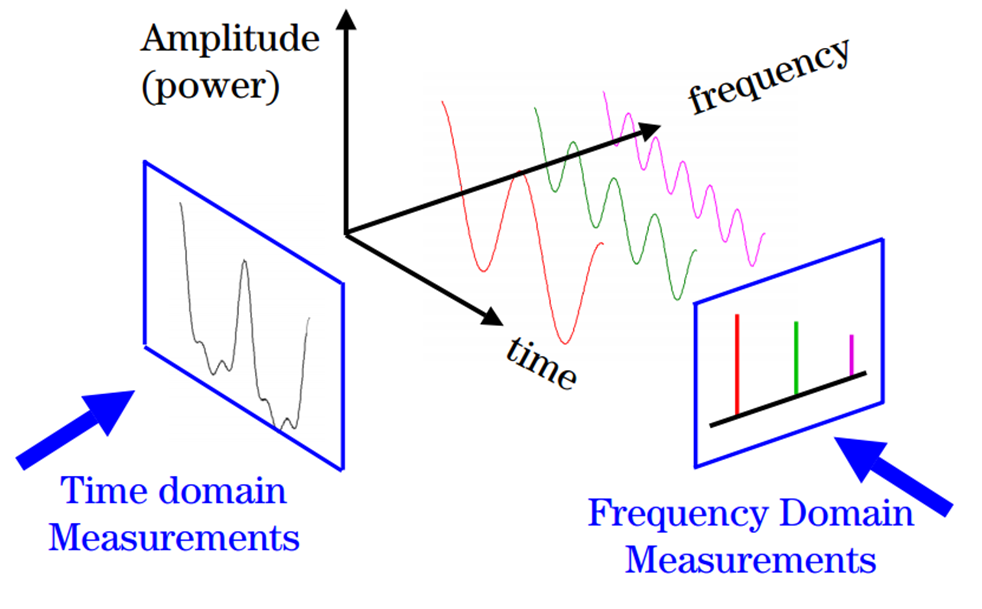
\includegraphics[width=4in]{amp-time-frequency}
	\caption{Conceptual comparison between time domain measurements (oscilloscope) and frequency domain measurements (spectrum analyzer)~\cite{thomas-sa}}
	\label{fig:amp-time-frequency}
\end{figure}

Fig.~\ref{fig:sa-screen} shows a screen capture of a typical spectrum analyzer measurement. The horizontal axis is frequency and the vertical axis is signal power in dB scale. This figure shows a fairly narrow band signal at 1.8271\,GHz. The power of the signal is 2.06\,dBm.

\begin{figure}[h]
	\centering
	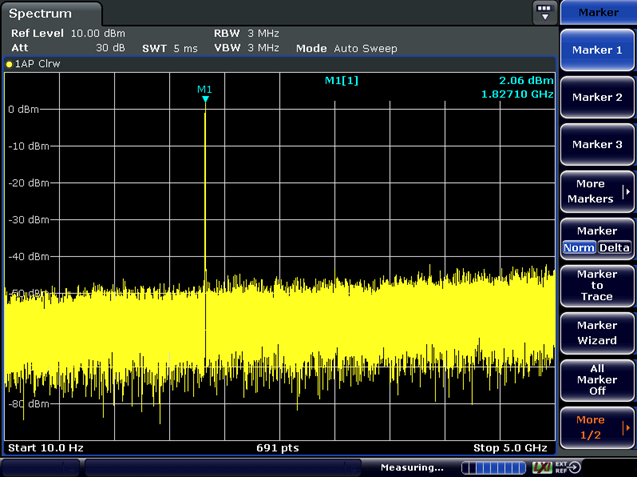
\includegraphics[width=4in]{sa-screen}
	\caption{Simplified block diagram of a spectrum analyzer.}
	\label{fig:sa-screen}
\end{figure}

At other frequencies where there is no input signal, we can still observe some measurement. As you might have guessed, these signals represent the noise, both from the signal source and from the spectrum analyzer itself. Obviously, it is important to have as low of a noise level as possible in order to detect extremely weak input signals. In fact, an important metric of a spectrum analyzer's performance is its sensitivity, i.e. the weakest signal that it can measure. This is often specified as \textit{Displayed Average Noise Level} (DANL), usually measured in dBm at the smallest \textit{resolution bandwidth} (RBW, we will come to this soon), or directly in dBm/Hz. The sensitivity is then simply DANL+SNR, where SNR is the minimum required \textit{signal to noise ratio}. For a top of the line spectrum analyzer, you can expect a DANL of close to -170\,dBm/Hz.

Another related metric is the \textit{dynamic range}, which refers to the power difference between the strongest and the weakest signal a spectrum analyzer can measure. Dynamic range is usually specified in dB. The absolute maximum dynamic range that a spectrum analyzer can achieve is the difference between the maximum allowable input power and the DANL. 
Sensitivity and dynamic range speak for the design and build quality of a spectrum analyzer. However, the achievable sensitivity and dynamic range in an actual measurement are usually lower than the maximum. It depends on what you want to measure and how you set up the spectrum analyzer. To understand this, we need to learn a bit more about how a spectrum analyzer works. 

The basic working principle of a typical spectrum analyzer is conceptually quite simple\footnote{The actual implementation of an instrument grade spectrum analyzer can be extremely complex to meet the high performance specs}. It is basically a glorified high frequency signal receiver. Fig.~\ref{fig:sa-blocks} shows a very simplified system diagram of a typical spectrum analyzer, highlighting its major blocks. The input signal is downconverted to a much lower frequency (usually several MHz) before it is captured by a power detector. The downconverter is represented by a mixer with a sweeping local oscillator (LO). The LO signal is swept through a span of frequency that can be set by the user; this sets the frequency span of the measurement. The downconversion of the signal allows it to be optimally conditioned for the detection circuitry. 

\begin{figure}[h]
	\centering
	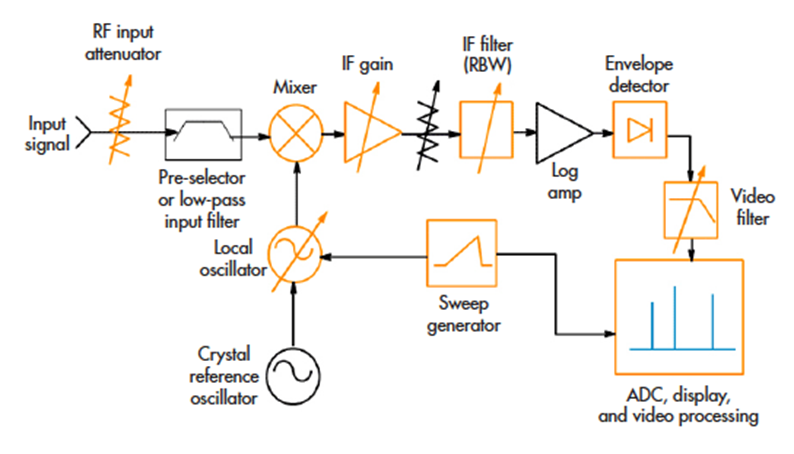
\includegraphics[width=4in]{sa-blocks}
	\caption{Simplified block diagram of a spectrum analyzer~\cite{diez-sa}.}
	\label{fig:sa-blocks}
\end{figure}

Before the downconverted signal enters the power detector, a narrow-band filter is used to allow only the desired signal to pass. This filter not only eliminates spurious signals but also limits the amount of noise power that enters the detector. As you can imagine, the narrower the filter passband is, the lower the noise floor would be. This filter is called the IF filter, and its bandwidth is called the resolution bandwidth (RBW). The power detector is effectively detecting the total power (signal plus noise) inside the resolution bandwidth. The best sensitivity and dynamic range of a spectrum analyzer can only be achieved with the narrowest RBW that is available in the instrument. Therefore, the available RBW bandwidth becomes an important metric itself. 

Besides affecting the noise floor, the RBW also has implications on how the signal looks on the screen. Consider the case of an ideal single-tone (meaning single frequency) input signal. The spectrum of this signal should look like a delta function in the frequency domain. Now imagine the receiver of the spectrum analyzer sweeps through the center frequency of the signal. Due to the finite width of the RBW, the measured spectrum will actually take the shape of the RBW filter! By carefully taking into the account of the RBW filter frequency response, the measured signal power and frequency can still be reconstructed. However, you would not be so lucky if you are dealing with more than one signal. Fig.~\ref{fig:sa-rbw} shows a scenario where three closely located signals cannot be reliably discerned by a large RBW. 

\begin{figure}[h]
	\centering
	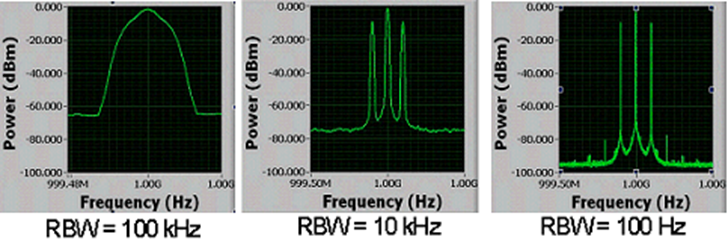
\includegraphics[width=4.5in]{sa-rbw}
	\caption{Small RBW resolves closely located signals.}
	\label{fig:sa-rbw}
\end{figure}

It becomes clear that an infinitely narrow IF filter is needed to faithfully reconstruct the true spectrum of the input signal. Obviously such a filter does not exist, and you will always have to keep in mind the broadening of the spectrum in a spectrum analyzer measurement. 

This simplistic introduction to spectrum analyzers will end here. There is obviously much more to learn about this fundamental high frequency signal characterization tool. To get a deeper understanding of spectrum analyzers and the principles of spectrum analysis, the following documents are recommended as further reading materials. 

\begin{itemize}[itemsep=0.1ex]
	\item ``Spectrum analysis basics,'' Agilent application note AN-150.
	\item ``Fundamentals of Real-Time Spectrum Analysis,'' Tektronix application note.
	\item Rigol DSA1030A-TG3 spectrum analyzer review and experiments (Video\footnote{This Youtube channel features many great tutorial videos related to high frequency electronics.}):\\  \url{https://www.youtube.com/watch?v=lu2Uaj3ZcoA }
\end{itemize}

\subsection{Coaxial RF Connectors}
As we learned in the introductory engineering electromagnetics course, electrical connections between high frequency circuit components may not be as simple as in the case of low frequency circuits. We have to consider wave propagation effects (transmission line effects) when the length of the connection is comparable with the wavelength. As a consequence, we have to consider impedance matching between the transmission lines and the circuit components. To make things simple, we often conform to a single impedance value, often called the system impedance, in an RF system. In most systems, this impedance value is \SI{50}{\ohm}\footnote{Why 50 Ω? read the following: \url{http://www.belden.com/blog/broadcastav/50-ohms-the-forgotten-impedance.cfm}}. 

Perhaps the most prevalent transmission line for medium to low-power RF/microwave systems is the coaxial cable, which consists of an inner conductor and an outer conductor arranged in a cylindrical fashion. Coaxial cables are great because they are generally low loss, can be made flexible, and provide great shielding/isolation of the signal being transmitted. In order to connect coaxial cables to an RF block, a coaxial RF connector is usually used. 

RF connectors comes in many different standards. They vary in shape, usable frequency range, signal attenuation, power handling, durability, etc. Fig.~\ref{fig:connectors} provides a glimpse of some common RF connectors. 

\begin{figure}[h]
	\centering
	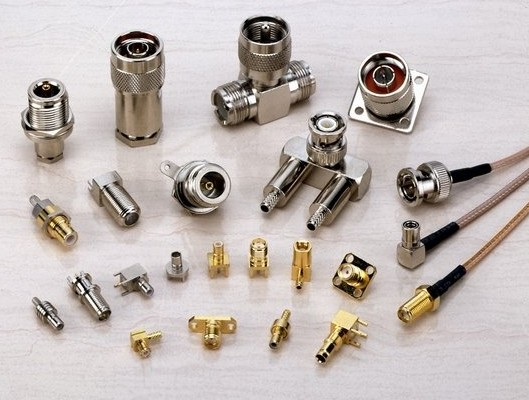
\includegraphics[width=4in]{connectors}
	\caption{Typical RF connectors. Source: \url{http://www.szelins.com/RF_Connector.html}}
	\label{fig:connectors}
\end{figure}

To learn about RF coaxial connectors, go through the following materials. 

\begin{itemize}[itemsep=0.1ex]
	\item ``Guidance Selecting Handling Coaxial RF Connectors,'' Rohde \& Schwarz.
	\item RF and microwave connector handling and care (Video): \url{https://www.youtube.com/watch?v=IOoSsvprpTg}
\end{itemize}

\newpage
\reversemarginpar
\marginnote{\textbf{Pre-lab Assignment}\\\textbf{2.1} \\Due: \due{Oct.~20th, 2016}}  

Please review EEC134 Lecture Note 3 and answer the following questions:
\begin{enumerate}[itemsep=0.1ex, label=\alph*)]
	\item A 10\,dBm 2.4\,GHz RF signal is sent through a \SI{50}{\ohm} TEM transmission line to a \SI{50}{\ohm} load. Assuming that the source impedance is also \SI{50}{\ohm}, what is the RMS voltage on the transmission line (i.ebetween the transmission line's signal and ground)?
	
	\item An RF signal of 0\,dBm power is amplified by an amplifier with 14\,dB power gain. The source impedance of the input signal is \SI{50}{\ohm} and is well matched with the input impedance of the amplifier. The output of the impedance of the amplifier is \SI{200}{\ohm} and is also well matched with a \SI{200}{\ohm} load. What's the voltage swing at the output of the amplifier?
	
	\item A transmission line of characteristic impedance $Z_t$ and length $l$ is connected to a load impedance of $Z_0$. What is the reflection coefficient at the input of the transmission line for the following conditions? What observation can you make? 
		\begin{enumerate}[label=\roman*)]
			\item $Z_t = 5 Z_0$, $l = 0.5\lambda$;
			\item $Z_t = 5 Z_0$, $l = 0.25\lambda$;
			\item $Z_t = 5 Z_0$, $l = 0.1\lambda$;
			\item $Z_t = 5 Z_0$, $l = 0.05\lambda$;
			\item $Z_t = 5 Z_0$, $l = 0.01\lambda$;
			\item $Z_t = 0.2 Z_0$, $l = 0.5\lambda$;
			\item $Z_t = 0.2 Z_0$, $l = 0.25\lambda$;
			\item $Z_t = 0.2 Z_0$, $l = 0.1\lambda$;
			\item $Z_t = 0.2 Z_0$, $l = 0.05\lambda$;
			\item $Z_t = 0.2 Z_0$, $l = 0.01\lambda$;
		\end{enumerate}
	
	\item A signal is sampled at frequency $F_s$ (in unit of samples per second). $N$ samples have been collected. When an FFT is performed on the samples, what is the resulting frequency resolution?
	
	\item An RF amplifier has a noise figure of 2\,dB. If an input signal with a signal to noise ratio (SNR) of 20\,dB is fed into the amplifier, what is the SNR of the output signal?
	
	\item What connectors are mechanically compatible with the 3.5\,mm type connectors? Which of these connectors has the largest operating frequency range?

\end{enumerate}

\reversemarginpar
\marginnote{\textbf{Pre-lab Assignment}\\\textbf{2.2} \\Due: \due{Oct.~27th, 2016}}  Please answer the following questions:
\begin{enumerate}[itemsep=0.1ex, label=\alph*)]
		
	\item Two RF amplifiers are cascaded as shown in Fig.~\ref{fig:cascade}. What is the total gain of the cascade? What is the total noise figure? 
	\begin{figure}[h]
		\centering
		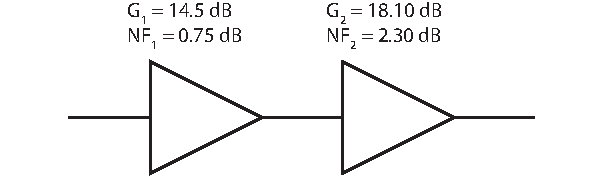
\includegraphics[width=4in]{cascade}
		\caption{A cascade of two RF amplifiers.}
		\label{fig:cascade}
	\end{figure}
		
	\item An RF amplifier has an input-output voltage relationship of the following:
		\[
			v_o = 10 v_i + 0.2 v_i^2 - 0.05 v_i^3,
		\]
		where $v_o$ is the output voltage and $v_i$ is the input voltage. Assume that the amplifier is well matched at the input and output to \SI{50}{\ohm} loads. 
		
		\begin{enumerate}[label=\roman*)]
			\item Calculate the output 1\,dB compression point P1dB;
			\item Calculate the output 3rd order intercept point OIP3;
			\item \st{Calculate the output 2nd order intercept point OIP2}.
		\end{enumerate}

	\item The Y-factor method is used to measure the equivalent noise temperature of a component, with a hot load of $T_1 = 320$\,K and cold load of $T_2 = 77$\,K. If the Y-factor ratio is measured to be 0.608\,dB, what is the noise figure of the component under test?
	
	\item What is the typical input IP3 of the Mini-Circuits GALI-84+ amplifier at 2\,GHz?
	
	\item What is the lowest noise figure 2.4\,GHz SMD RF amplifier you could find? 

\end{enumerate}

\newpage
\section{Equipment \& \\Supplies}

\begin{itemize}[itemsep=0.5ex]
\item 2 $\times$ Mini-Circuits ZX60-272LN-S+ amplifier (Fig.~\ref{fig:amp-pic}). Table shows its main specifications (typical values) at room temperature. More detailed specifications can be found in the datasheet (\url{http://www.minicircuits.com/pdfs/ZX60-272LN+.pdf}\footnote{\textbf{It is always a good idea to read the datasheet before using a component.}}).

\begin{figure}[h]
	\centering
	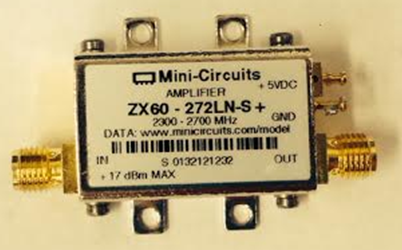
\includegraphics[width=2in]{amp-pic}
	\caption{Picture of the Mini-Circuits ZX60-272LN-S+ amplifier.}
	\label{fig:amp-pic}
\end{figure}

\begin{table}[h]
	\centering
	\caption{ZX60-272LN-S+ Typical Specifications.}
	\renewcommand{\arraystretch}{1.2}
	\begin{tabular}{|c|c|}
		\hline  Frequency range & 2300 -- 2700\,MHz \\ 
		\hline  Noise figure & 0.8\,dB \\ 
		\hline  Gain & 14\,dB \\ 
		\hline  P1dB & 18.5\,dBm\\ 
		\hline  OIP3 & 31.5\,dBm \\ 
		\hline  Input VSWR & 1.2 \\ 
		\hline  Supply voltage & 5\,V \\ 
		\hline  Supply current & 55\,mA \\ 
		\hline 
	\end{tabular} 
\end{table}

\item 1 $\times$ Mini-Circuit ZX10-2-332-S+ power splitter/combiner. An RF power splitter is used to evenly split the RF power from the input port (marked ``S'') into two output ports (marked ``1'' and ``2''). However, here we will use it as a power combiner\footnote{You will learn in an RF circuit design class that most passive RF components --- splitter is one of them --- are reciprocal, meaning that you use their output as input and vice versa.}, which combine the signals from two output ports into the input port. 

\begin{figure}[h]
	\centering
	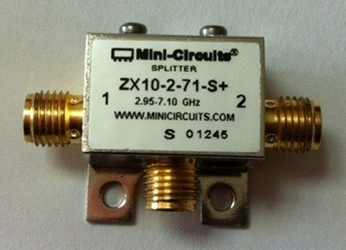
\includegraphics[width=2in]{splitter-pic}
	\caption{Picture of the Mini-Circuits ZX10-2-332-S+ amplifier.}
	\label{fig:splitter-pic}
\end{figure}

\item 1 $\times$ Mini-Circuits VAT-3+ 3\,dB RF attenuator. As its name suggests, the attenuator attenuates the RF signal by 3\,dB. 

\item GW-Instek GSP-730 spectrum analyzer (Fig.~\ref{fig:gsp730}). The GSP-730 is a low-cost 3\,GHz spectrum analyzer. It doesn’t have the best performance~\footnote{We've chosen this spectrum analyzer primarily for cost reasons.}, but we will work around the limitations to make it useful for our labs. The GSP-730 can be remotely controlled from the lab computer by the GGT software provided by GW-Instek. 

The spectrum analyzers are usually locked in the Kemper 2112 cabinet. However, your group can check one out if you wish to use it outside of lab hours. The GSP730 will fit in your EEC134 toolbox.

\begin{figure}[h]
	\centering
	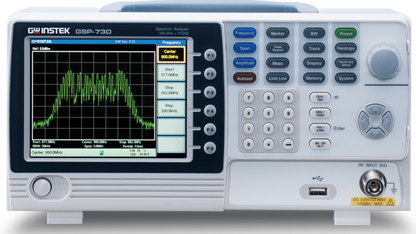
\includegraphics[width=3in]{gsp730}
	\caption{Picture of the Instek GSP730 spectrum analyzer.}
	\label{fig:gsp730}
\end{figure}
 
\item 2 $\times$ TPI synthesizers (Fig.~\ref{fig:tpi-synth}) and 2 $\times$ USB-mini cables. The TPI synthesizer is a low-cost RF signal generator based on the Analog Devices AD4351 single-chip synthesizer. The synthesizers will be distributed to each group and it will be your responsibility to keep them safe. 

Note that every TPI synthesizer is calibrated and has its individual serial number. When you connect the synthesizer to a computer through the USB-mini cable, a window will pop up to let you select the calibration file based on the serial number. 

\begin{figure}[h]
	\centering
	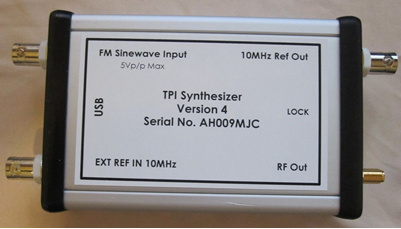
\includegraphics[width=3in]{tpi-synth}
	\caption{Picture of the TPI v4 RF synthesizer.}
	\label{fig:tpi-synth}
\end{figure}

\item 2 $\times$ 12" and 2 $\times$ 6" semi-flex coaxial SMA cables. The coaxial cables can be bent to a certain extent, but please do not bend them excessively. 

\begin{figure}[h]
	\centering
	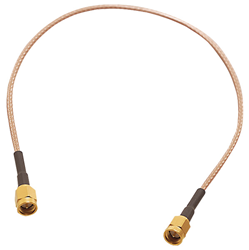
\includegraphics[width=1.5in]{rf-cable}
	\caption{Picture of the semi-flex coaxial cable.}
	\label{fig:rf-cable}
\end{figure}

\item 1 $\times$ TNC (male) to SMA (female) connector. 

\begin{figure}[h]
	\centering
	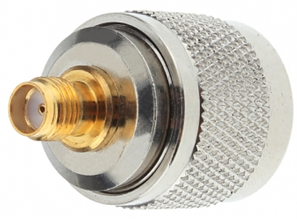
\includegraphics[width=1.5in]{tnc-sma}
	\caption{Picture of the TNC (male) to SMA (female) connector.}
	\label{fig:tnc-sma}
\end{figure}

\end{itemize}


\newpage
\section{Procedures}

\subsection{Getting to know your equipment}
\label{sec:equipment}

In this lab, we will measure the frequency and power of an RF signal generated by the TPI synthesizer with the GSP-730 spectrum analyzer. The measurement set up is shown in Fig.~\ref{fig:setup-single-tone}.

\begin{figure}[h]
	\centering
	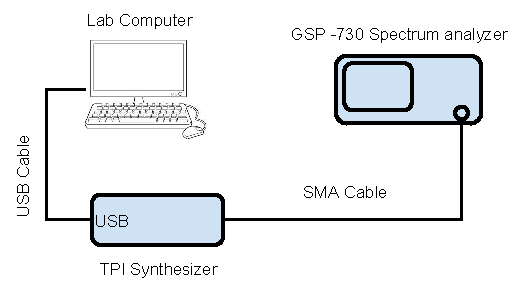
\includegraphics[width=3.5in]{setup-single-tone}
	\caption{Testing the TPI synthesizer and the GSP-730 spectrum analyzer.}
	\label{fig:setup-single-tone}
\end{figure}

\begin{enumerate}
	\item Connect the TNC-male to SMA-female adapter to the input port of spectrum analyzer (labeled ``RF INPUT \SI{50}{\ohm}''). Follow proper handling guidelines (in this case, hold the SMA-female end still and rotate only the TNC jacket). The adapter should be left on the spectrum analyzer from now on. 
	
	\item Connect the output of the TPI synthesizer to the input of the spectrum analyzer (with the adapter already connected) using an SMA cable.
	
	\item Connect the TPI synthesizer to the lab computer using an USB cable (provided with the kit).
	
	\item Turn on the spectrum analyzer and configure it as below.
		\begin{enumerate}
			\item Press the ``Preset'' button. \textbf{Always} preset the spectrum analyzer before starting a new experiment.
			
			\item Set the center frequency. Press the blue ``Frequency'' button, then press the ``F1'' button to select the ``Center'' frequency option. Type in ``2.4 GHz'' using the numerical panel on the spectrum analyzer. 
			
			\item Set the frequency span.  Press the blue ``Span'' button, then press ``F1'' button to select the ``Span'' option. Type in ``20 MHz''. Now you should be able to observe the frequency range from 2.39\,GHz to 2.41\,GHz\footnote{You can also achieve this by setting the ``Start frequency'' and ``Stop frequency''; play with it.}. 
			
			\item Set the reference level. Press the ``Amplitude'' button, then press ``F1'' button to select the ``Ref. Level'' option. Type in ``20 dB'' to set the reference level to 20\,dBm\footnote{The reference level is set to be comparable to the signal input power.} . The screen of the spectrum analyzer should look like that in Fig.~\ref{fig:sa-reference}. 
				\begin{figure}[h]
					\centering
					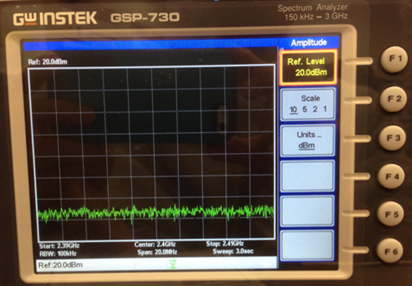
\includegraphics[width=3in]{sa-reference}
					\caption{Setting the reference level.}
					\label{fig:sa-reference}
				\end{figure}
		\end{enumerate}
		
	\item Measuring a single-tone RF signal
		\begin{enumerate}
			\item Launch the \textit{SynthMachine} software and choose the appropriate calibration file (serial number) for the TPI synthesizers. In the SynthMachine software, set the ``Center Frequency'' to 2400\.MHz , set the ``Output Power'' to 10\,dBm, and click ``RF On'' to turn on the RF signal output. 
				\begin{figure}[h]
					\centering
					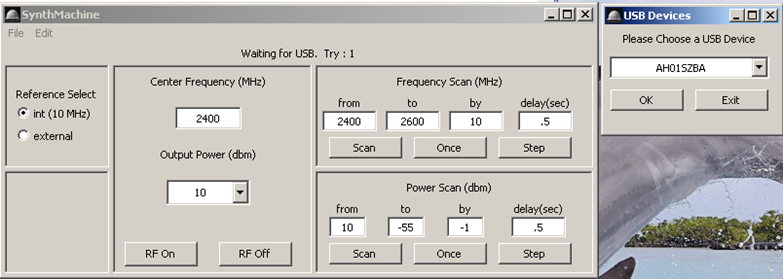
\includegraphics[width=5in]{synth-machine}
					\caption{Screenshot of the SynthMachine software.}
					\label{fig:synth-machine}
				\end{figure}
							
			\item Observe the spectrum analyzer screen. It should look like the following. 
				\begin{figure}[h]
					\centering
					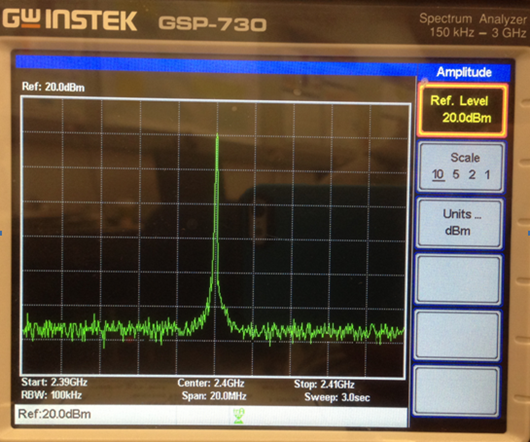
\includegraphics[width=3in]{sa-single-tone}
					\caption{Screenshot of the spectrum analyzer with a single-tone input.}
					\label{fig:sa-single-tone}
				\end{figure}		
									
			\item Press the gray ``BW'' (meaning bandwidth) button to go into the resolution bandwidth menu. Press ``F1'' to set the RBW to manual mode. Three possible RBW options should now appear in the sidebar menu. Capture the screen for each of the three settings\footnote{You can capture the screen by a camera or using the remote control software GGT. The software can be launched from the Start Menu of the lab computer. We'll leave it to you to explore how to capture the screen using the software.}. In your lab report, describe the differences between the three screen captures and explain why such differences exist.
							
			\item Set the RBW to the smallest possible value.
							
			\item Press the ``Peak Search'' button, and a marker is automatically located at the RF signals. You can read the frequency and power values of this marker at the right upper corner of the screen. Record the power of this signal. How does it compare it with the output setting of the TPI synthesizer? Assume that the TPI synthesizer output power is accurate, what do you think is the cause of the difference? This measured signal power which we will designate as $P_{cal}$ will be used as a reference for later labs.		
		\end{enumerate}	
		
	\item Observing the harmonics. 
		\begin{enumerate}
			\item Now set the output frequency of the TPI synthesizer to 800 MHz.
			
			\item Preset and configure the spectrum analyzer as follows: 
				\begin{enumerate}
					\item Start frequency = 500\,MHz; 
					\item Stop frequency = 3000\,MHz;
					\item RBW = auto;
					\item Reference level = 20\,dBm.
				\end{enumerate}
		\end{enumerate}	
	
	\item Measuring two RF signals. 
		\begin{enumerate}
			\item Turn off the RF power from the TPI synthesizer.  
			
			\item Disconnect the TPI synthesizer from the SMA cable.
			
			\item Connect the input port (labeled ``S'') of the splitter/combiner to the input of the spectrum analyzer with an SMA cable.
			
			\item Connect the output ports of the two synthesizers (labeled ``RF Out'') with the output ports of splitter/combiner (labeled ``1'' and ``2'') via male-male SMA adapters. Fig.~\ref{fig:setup-two-tone} shows the measurement setup. 
				\begin{figure}[h]
					\centering
					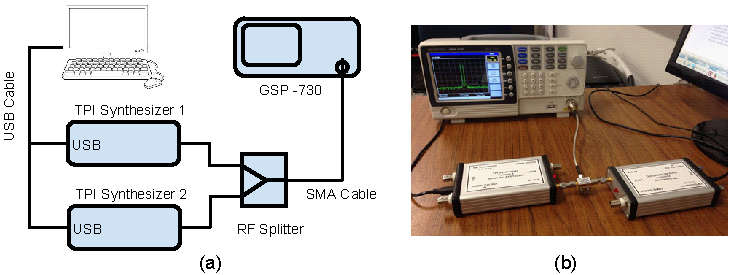
\includegraphics[width=5in]{setup-two-tone}
					\caption{Two-tone measurement setup.}
					\label{fig:setup-two-tone}
				\end{figure}			
			
			\item Preset the spectrum analyzer and configure it as below.
				\begin{enumerate}
					\item Center frequency = 2.4\,GHz;
					\item Span = 20\,MHz;
					\item RBW = 100\,kHz;
					\item Reference level = 20\,dBm.
				\end{enumerate}

			\item Launch another instance of the SynthMachine software (now you should have two instances of SynthMachine running) and choose the appropriate calibration file (serial number) for the second TPI synthesizer. Set the ``Center Frequency'' to 2400\,MHz for the first synthesizer and 2401\,MHz for the second. Set the ``Output Power'' to 10\,dBm for both synthesizers.
			
			\item Now turn on the TPI synthesizers by clicking the ``RF On'' buttons in both instances of the SynthMachine software. 
			
			\item The screen of the spectrum analyzer should look similar to Fig.~\ref{fig:sa-two-tone}. 
				\begin{figure}[h]
					\centering
					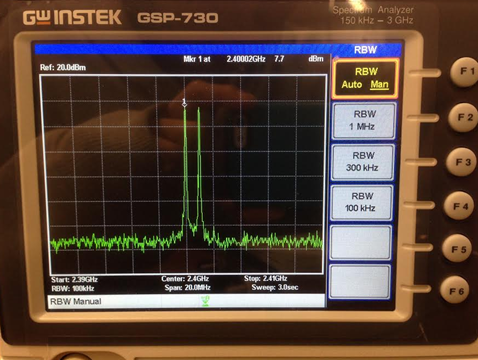
\includegraphics[width=3in]{sa-two-tone}
					\caption{Screenshot of the spectrum analyzer with two-tone input.}
					\label{fig:sa-two-tone}
				\end{figure}
			
			\item Set the RBW to the three possible manual options. Capture the screen for each of the three settings. Describe the differences between the three screen captures and explain why such differences exist in your lab report.
			
		\end{enumerate}
\end{enumerate}


\subsection{Characterizing the bandwidth and the gain}
\label{sec:bw-gain}

\begin{enumerate}
	\item Connect the output port of LNA (labeled ``OUT'') to one end of a 3-dB attenuator\footnote{The use of an attenuator here is to limit the RF power input to the spectrum analyzer for more accurate result. This should not be necessary on a better spectrum analyzer.}, then connect the other end of the attenuator to the spectrum analyzer with an SMA cable. 
	
	\item Connect the input port of the LNA to the TPI synthesizer via a SMA male-to-male connector. 
	
	\textbf{Note:} In general, always terminate the input and output ports of an RF amplifier before applying dc power. 
	
	\item Connect the ``+5VDC'' pin of the amplifier to the positive terminal of the lab power supply using a wire; connect the ``GND'' pin of the amplifier to the ground of the power supply. Fig.~\ref{fig:setup-bw-gain} shows the measurement setup. 
	
		\begin{figure}[h]
			\centering
			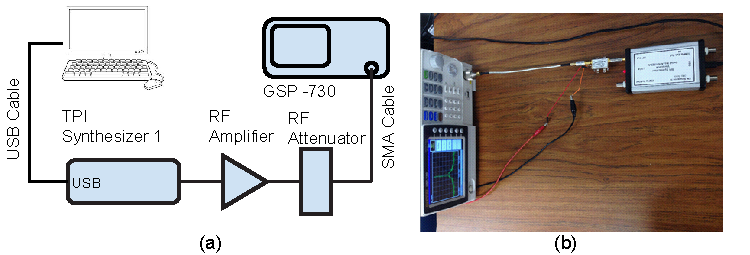
\includegraphics[width=5in]{setup-bw-gain}
			\caption{Amplifier bandwidth and gain measurement setup.}
			\label{fig:setup-bw-gain}
		\end{figure}	
	
	\item Preset the spectrum analyzer and configure it as below.
		\begin{enumerate}
			\item Center frequency = 2.4\,GHz; 
			\item Span = 4\,MHz;
			\item Reference level = -10\,dBm;
			\item RBW = auto.
		\end{enumerate}
	
	\item Configure the TPI synthesizer as follows:
		\begin{enumerate}
			\item Center Frequency = 2.4\,GHz;
			\item Output Power pout=  -25\,dBm.
		\end{enumerate}

	\item Set the power supply to output +5\,V. 

	\item Verify that the amplifier is drawing approximately 55\,mA of dc current. This indicates---to some extent---that the amplifier is working well and is not damaged. 
	
	\item Turn on the TPI synthesizer.
	
	\item You should now see a signal at 2.4\,GHz on the spectrum analyzer.

	\item Press the ``Peak Search”'' button on the spectrum analyzer, and a marker is automatically located at the desired signal. Let $P_{meas}$  be the measured signal power. 
	
	\item Calculate the gain of the amplifier. 
		\[
			G = P_{meas} - P_{out} - (P_{cal} - 10) + 3 \hspace{2.5em} \text{(dB).}
		\]
		
		Verify that this value agrees with the amplifier's datasheet. Explain why the above equation is used to calculate the gain. 
	
	\item Now sweep set the output frequency of the TPI synthesizer from 2.0\,GHz to 3.0\,GHz (include at least 8 data points) and measure the amplifier gain at each frequency. Note each time when you are changing the output frequency of TPI synthesizer, you also need to change the center frequency of spectrum analyzer, otherwise you won't observe any signals. Please note down the frequency and the measured power, then use the above formula to calculate the gain. Plot the gain with respect to frequency. Include at least 8 data points. What is the 3\,dB bandwidth of the amplifier? What is the maximum gain variation in the 2.3--2.7\,GHz range? Does the measured data agree well with the datasheet?
\end{enumerate}

\subsection{Measuring P1dB}
\label{sec:p1db}

Using the same setup as in Experiment.~\ref{sec:bw-gain}, we will measure the 1-dB compression point of the amplifier. 

\begin{enumerate}
	\item Preset and configure the spectrum analyzer as follows:
		\begin{enumerate}
			\item Center frequency = 2.4\,GHz;
			\item Span = 4\,MHz;
			\item RBW = auto;
			\item Reference level = -10\,dBm.
		\end{enumerate}
		
	\item Set the synthesizer output frequency to 2.4\,GHz.
	
	\item Set the output power of the TPI synthesizer from -20\,dBm to 10\,dBm in steps of 1\,dBm. Record the measured signal power (output of the amplifier) on the spectrum analyzer. Note when you increase the input power to some extent, the signal peak will be out of screen range, but you can always find the peak value by pressing the ``Peak Search'' button on the spectrum analyzer. Though you can adjust the reference level to a higher value to observe the signal peak, this change would lead to a poor measurement result.
	
	\item Plot the measured output power vs. the input power. What is the output 1\,dB compression point for the amplifier? Does it agree with the datasheet?
\end{enumerate}

\subsection{Measuring IP3}
\label{sec:ip3}

\begin{enumerate}
	\item For the IP3 measurement, we need two input signals with a slight frequency offset. Set up the measurement as illustrated by Fig.~\ref{fig:setup-two-tone-amp}.
		\begin{figure}[h]
			\centering
			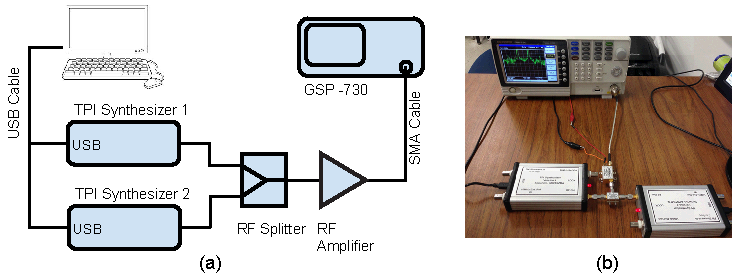
\includegraphics[width=4.5in]{setup-two-tone-amp}
			\caption{Amplifier IP3 measurement setup.}
			\label{fig:setup-two-tone-amp}
		\end{figure}
	
	\item Preset and configure the spectrum analyzer as follows:
		\begin{enumerate}
			\item Center frequency = 2.4005\,GHz;
			\item Span = 4\,MHz;
			\item RBW = auto
			\item Reference level = -20\,dBm.
		\end{enumerate}
	
	\item Configure the TPI synthesizers as follows:
		\begin{enumerate}
			\item Synthesizer 1:
				\begin{enumerate}
					\item Output frequency = 2.4\,GHz;
					\item Output power = -10\,dBm;
				\end{enumerate}
			\item Synthesizer 2:
				\begin{enumerate}
					\item Output frequency = 2.401\,GHz;
					\item Output power = -10\,dBm.
				\end{enumerate}
		\end{enumerate}
	
	\item The spectrum analyzer screen should look like the following. The fundamental signals will be beyond what the screen can display (Fig.~\ref{fig:sa-two-tone-amp}-b); we do this intentionally to keep the reference level small (-20 dBm) to obtain a better measurement result. You can use ``F1'' - ``F6'' key to locate every fundamental tone and 3rd order intermodulation (IM3) signals. 
		\begin{figure}[h]
			\centering
			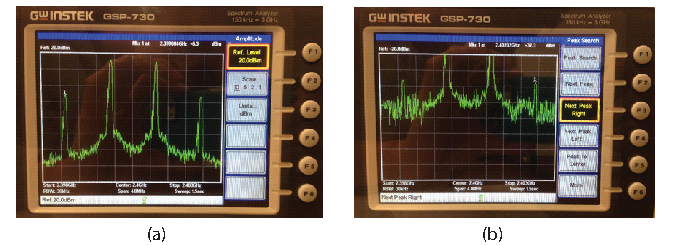
\includegraphics[width=4.5in]{sa-two-tone-amp}
			\caption{Screeshot of the amplifier two-tone measurement. (a) Low signal level; (b) High signal level.}
			\label{fig:sa-two-tone-amp}
		\end{figure}
	\item Sweep the output power of both TPI synthesizers from -25\,dBm to 5\,dBm. Record the measured fundamental and IM3 signal power. The two IM3 signals may exhibit different power levels. This may be caused by a number of reasons, such as gain variation and memory nonlinear effects. For this lab, simply pick one of the two IM3 signals.
	
	\item Plot the measured fundamental and IM3 signal power vs. the input power. What is the output IP3 (OIP3) point for the amplifier? Does it agree with the datasheet?

\end{enumerate}


\subsection{RF PCB designs}

\subsubsection{RF Amplifier PCB}
Design a test PCB for the ADI ADL5611 RF gain block IC. Before you start your design, it would be helpful to go through \href{https://github.com/ucdart/UCD-EEC134/blob/master/labs/appendices/kicad/pcb-tutorial.pdf}{Example 2 of the EEC 134 PCB Design Tutorial}. 

\begin{enumerate}
	\item Follow the recommended schematic and layout in the datasheet:\\ (\url{http://www.analog.com/static/imported-files/data_sheets/ADL5611.pdf} ). Your final circuit will look similar, but may not be identical to the ADL5611 evaluation board (Fig.~\ref{fig:adl5611-evalz}).
 
		\begin{figure}[h]
			\centering
			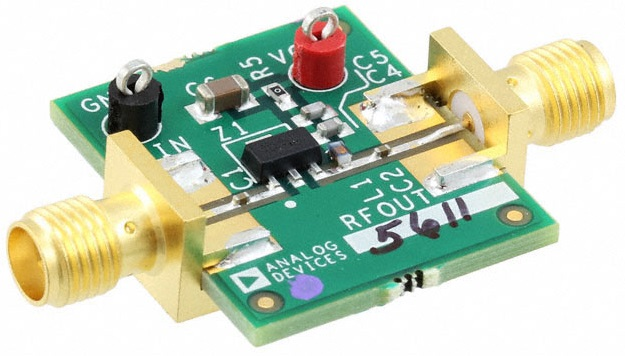
\includegraphics[width=2in]{adl5611-evalz}
			\caption{Evaluation board for ADI ADL5611.}
			\label{fig:adl5611-evalz}
		\end{figure}
	\item Use Bay Area Circuits as the PCB vendor. Your PCB design should conform to the Bay Area Circuits student specials specifications. 
	
	\item The PCB area should not exceed 1 $\times$ 1\,in$^2$.
	 
	\item Make sure that you have \SI{50}{\ohm} transmission lines for the input and output SMA connectors.
	
	\item The recommended footprint of the SMA connectors are available at this \href{https://github.com/ucdart/UCD-EEC134/blob/master/labs/lab2/resources/SMA%20Size.jpg}{link}. It is also available in the ``resources'' folder. 
	
	\item Use 0603 sized SMD resistors and capacitors. 
	
	\item The TA will provide the ADL5611 IC and SMA connectors. You will be responsible for acquiring the rest of the circuit components. Do remember to check the \href{https://docs.google.com/spreadsheets/d/1GJnBLUymuVzXjrK0Zkdbc2lwTbw0z9a0JR4bLLzO-Sw/edit#gid=4}{class inventory}. 
	
	\item The following items are due by \due{Oct.~30th, 2015}. Refer to Table.~\ref{tab:deliverables} for submission instructions. 
		\begin{itemize}
			\item A PCB design report to the TA. The design report should include the following:
				\begin{itemize}
					\item Bill of materials.
					\item Screen capture of the schematic.
					\item Screen capture of the PCB layout.
					\item Bay Area Circuit design for manufacturing (DFM) report from showing no errors.
				\end{itemize}
			\item A PCB review report to the TA. The review report should be completed by a different team than yours. You will be responsible for finding this review team. The review report should follow the general guideline of the PCB Review Report Template.
			
			\item PCB output (Gerber) files.
		\end{itemize}

	\item After the PCB comes back, you will need to assemble the circuit and test it. The tests would be similar to what you have done in Measurement~\ref{sec:equipment}--\ref{sec:ip3}. Test report for this PCB is due by \due{Nov.~20th, 2015}.

\end{enumerate}
	
\subsubsection{RF variable attenuator PCB}
Design a test PCB for the Skyworks SKY12322-86LF variable attenuator. 

\begin{enumerate}
	\item Follow the recommended schematic (Fig.~8) in the datasheet:\\ (\url{http://www.skyworksinc.com/uploads/documents/200218C.pdf}). 
	
	Fig.~7 of the datasheet shows the layout of the SKY12322-86LF evaluation board. However, your PCB design doesn't need to be this big.

	\item The PCB area should not exceed 1 in $\times$ 1 in.	

	\item You should use your Teensy micro-controller for setting the attenuation level. Note that the Teensy digital pins have \href{https://www.pjrc.com/teensy/td_digital.html}{internal pull-up resistors}. 
	
	\item Use Bay Area Circuits as the PCB vendor. Your PCB design should conform to the Bay Area Circuits student specials specifications. 
	
	\item Make sure that you have \SI{50}{\ohm} transmission lines for the input and output SMA connectors.
	
	\item The TA will provide the SKY12322-86LF IC and SMA connectors. You will be responsible for acquiring the rest of the circuit components. Do remember to check the \href{https://docs.google.com/spreadsheets/d/1GJnBLUymuVzXjrK0Zkdbc2lwTbw0z9a0JR4bLLzO-Sw/edit#gid=4}{class inventory}. 
	
	\item The following items are due by \due{Nov.~6th, 2015}. Refer to Table.~\ref{tab:deliverables} for submission instructions. 
		\begin{itemize}
			\item A PCB design report to the TA. The design report should include the following:
				\begin{itemize}
					\item Bill of materials.
					\item Screen capture of the schematic.
					\item Screen capture of the PCB layout.
					\item Bay Area Circuit design for manufacturing (DFM) report showing no errors.
				\end{itemize}
			\item A PCB review report to the TA. The review report should be completed by a different team than yours. You will be responsible for finding this review team. The review report should follow the general guideline of the PCB Review Report Template.
			
			\item PCB output (Gerber) files.
		\end{itemize}

	\item After the PCB comes back, you will need to assemble the circuit and test it. The main test is the attenuation level at various attenuation settings. Test report for this PCB is due by \due{Nov.~27th, 2015}.

\end{enumerate}

\begin{thebibliography}{9}
 
\bibitem{thomas-sa}
Jeff Thomas, Tom Holmes, Terri Hightower, ``Learn RF Spectrum Analysis Basics,'' Agilent Technologies, \url{https://www.jlab.org/uspas11/Reading/RF/RF%20Spectrum%20Analysis.pdf}.

\bibitem{diez-sa}
Erik Diez, ``The Fundamentals of Spectrum Analysis,'' Agilent Technologies, \url{http://electronicdesign.com/test-amp-measurement/fundamentals-spectrum-analysis}.


\end{thebibliography}

\end{document}